\chapter{Introduction}
\label{C:introduction}

Today, the ATM swallowed my card and put my balance in arrears.
Or perhaps yesterday, I don't remember.
I must have done something wrong.
Machines don't just take people's money for no reason. 
I must have chosen the wrong option.
Perhaps it was yesterday.

It is hard to imagine spending a day without interacting with software in some way.
Most of the software I touch is fairly innocuous, where an error might cause a few minutes' grumbling, but no real heartache.
For other software, such as the banking server at my building society, or the cruise control on my car, errors can be disastrous.
Unfortunately, the level of \emph{trust} provided to software does not generally coincide with the \emph{effort} taken to ensure correctness of that software.
When banking software goes awry, people suffer financially.
When debt recovery software goes awry, people suffer emotionally.
When car software goes awry, people suffer physically.
It is hard to imagine spending a day without software going awry in some way.

What really makes this topic frustrating is that these are, in some sense, solved problems.
We know how to write correct software, or at least we know how to write \emph{more} correct software.
With formal methods we can prove that a program acts in accordance with some high-level specification.
With type systems we can rule out whole classes of bugs and vulnerabilities just by compiling and typechecking the program.
With high-level languages and high-level abstractions we can write programs that are more ``obviously correct'' and easier to reason about.

Why do these problems persist?
Part is the effort required: there is a real cost to proving programs correct using formal methods.
Another part is lack of education and inertia.
However, the part I wish to focus on is the performance costs associated with high-level abstractions.

Compared to traditional imperative languages such as C, Java or Go, high-level languages with static type systems (Haskell being a notable example) reach a sweet middle ground in terms of effort to correctness.
While they do not ensure the complete correctness that formal methods promise, they still provide valuable guarantees about the absence of particular errors.

While my motivation for this thesis is born of a deep discontent with computing, the actual goal of this thesis is to improve the performance of certain programs.
If we were able to rule out a large class of errors and offer competitive performance, surely this would reduce at least \emph{one} of the barriers to writing correct programs.
One can hope.

\section{Fusion}

Suppose we have an array and wish to perform two operations on it: first, we want to create a new array with the elements above zero, and secondly we want to find the maximum element.
We can write this as follows using the combinators @filter@ and @maximum@:

\begin{code}
filterMax (input : Array Int) : (Array Int, Int)
 = let above = filter (>0) input
       max   = maximum     input
   in (above, max)
\end{code}

\begin{figure}
\center
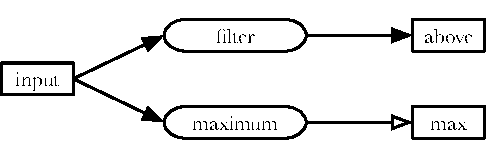
\includegraphics{figs/combinators/filtermax.pdf}
\caption[Combinator diagram for filterMax]
{Combinator diagram for computing filter and maximum of the same input array.
On the left is the manifest input array called `input', denoted by a sharp-cornered rectangle.
The input array feeds into two combinators, filter and maximum, denoted by round-cornered rectangles.
The output of each combinator is stored in a manifest array called `above' for the filter, and a manifest scalar called `max' for the maximum.}
\label{fig:combinators:filtermax}
\end{figure}


\autoref{fig:combinators:filtermax} shows the combinator diagram for this example.
The stored arrays and scalars (input, above and max) are shown as sharp-cornered rectangles to denote that they are `manifest': they are stored in memory.
Combinators which perform operations (filter and maximum) are round-cornered rectangles.
Edges in this graph denote the flow of data between nodes.
The edge between maximum and max uses an unfilled arrowhead, denoting that this is a \emph{fusion-preventing} edge, because maximum cannot know its output value until it has seen all the elements of the array.
That is, maximum must see the end of the array before producing any output.
We call combinators with fusion-preventing output edges \emph{offline} and those with fusible outputs \emph{online}.
In many cases, combinators that produce scalar outputs (maximum, minimum, sum, mean) offline, while combinators that produce arrays (filter, map) are online; however this is not always true: the `sort' combinator produces an array but is offline, as all the data needs to be seen before it can be sorted.


The definition above is small and neat, and computes the right value, but is it fast?
A naive way of executing this program is to loop over the input array performing the filter, then start from the start again to compute the maximum.
The combinator diagram in \autoref{fig:combinators:filtermax-stream} shows the \emph{clustering} where the filter and the maximum are computed in different loops.

However, if the array is large, this extra loop can take a lot of time.
Ideally we would perform both computations in a single loop: the clustering in \autoref{fig:combinators:filtermax-fused}.
There are two possible ways to run this program: by computing the filter and the maximum in separate loops, 
How many loops are in this program? We don't know - it depends on whether the compiler is able to fuse these together.
Furthermore, the only way to tell is by inspecting the compiler output.
One way to be sure about is by writing it yourself.
The code we want to run is more like this:

\begin{code}
filterMax (input : Array Int) : (Array Int, Int)
 = loop 0 Array.empty 0
 where
  loop index above max
   | index == Array.length input
   = (above, max)
   | otherwise
   = let element = Array.index input index
         above'  = if element > 0
                   then Array.snoc above element
                   else above
         max'    = if element > max
                   then element
                   else max
     in  loop (index + 1) above' max'
\end{code}




\begin{figure}
\center
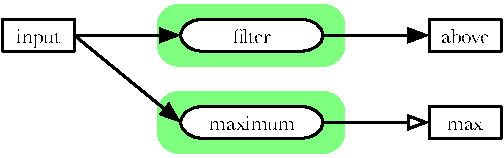
\includegraphics{figs/combinators/filtermax-stream.pdf}
\caption{Stream fusion requires two loops for the FilterMax example, because the input array is used twice.}
\label{fig:combinators:filtermax-stream}
\end{figure}

\begin{figure}
\center
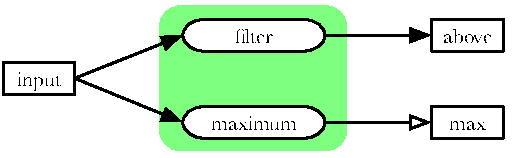
\includegraphics{figs/combinators/filtermax-fused.pdf}
\caption{Process fusion is able to fuse FilterMax into a single loop.}
\label{fig:combinators:filtermax-fused}
\end{figure}

The mapPairs function takes an array of pairs, and applies f to the first elements and g to the second elements.
This can be written by unzipping the array of pairs into two arrays, then mapping both arrays, then zipping the arrays back together.
However, stream fusion is unable to fuse this together and results in the clustering in \autoref{fig:combinators:mappairs-zip}.

\begin{code}
mapPairs (f : a -> c) (g : b -> d) (abs : Array (a,b)) : Array (c,d)
 = let (as,bs) = unzip abs
        cs     = map f as
        ds     = map g bs
   in  zip cs ds
\end{code}

This can be rewritten as a single map with the arrow combinator @(f *** g)@, which applies f to the first element and g to the second.
This single map is fused together by construction, and has the clustering in \autoref{fig:combinators:mappairs-arrow}.

\begin{code}
mapPairs (f : a -> c) (g : b -> d) (abs : Array (a,b)) : Array (c,d)
 = map (f *** g) abs
\end{code}

\begin{figure}
\center
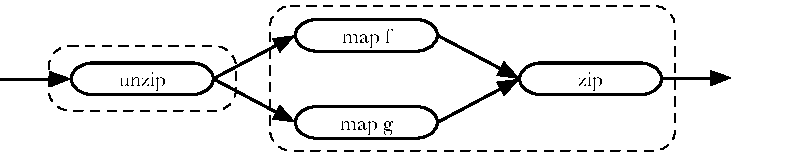
\includegraphics{figs/combinators/mappairs-zip.pdf}
\caption{Map pairs}
\label{fig:combinators:mappairs-zip}
\end{figure}

\begin{figure}
\center
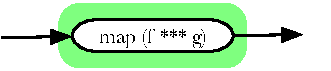
\includegraphics{figs/combinators/mappairs-arrow.pdf}
\caption{Map pairs manually fused together}
\label{fig:combinators:mappairs-arrow}
\end{figure}

\section{Process fusion}

Process fusion is able to fuse the above examples by treating each combinator and array as a sequential process, and the group of combinators as a concurrent process network.
Fusion then becomes the problem of finding a sequential interleaving of the process network that executes with bounded buffers.
In this way, we can abstractly treat processes as running concurrently, but once fusion occurs, there will be no concurrency overhead.

The filterMax example from before now becomes a process network, where we explicitly convert the input array to a stream, and back.
There is a bit more boilerplate around converting to and from arrays, but otherwise it is more or less faithful to the original version.
\begin{code}
filterMax :: Array Int -> Network (Array Int, Int)
filterMax inputArray
 = do input  <- streamOfArray  inputArray

      above  <- filter (>0)    input
      max    <- maximum        input

      aboveA <- arrayOfStream  above
      maxA   <- scalarOfStream max
      return (aboveA, maxA)
\end{code}

The streamOfArray is its own process, which converts an input array to a stream or `Channel'.
\begin{code}
streamOfArray :: Array a -> Network (Channel a)
streamOfArray input
 = do ys <- output
      process (read 0)
       { read i = Case (i < Array.length input) (push i) done
       , push i = Push ys (Array.index input i) (read (i + 1))
       , done   = Done
       }
      return ys
\end{code}

This creates a new output channel, @ys@, to which the output will be pushed.
A process may push to any number of channels at different rates, so creating the output channel is a separate step.
It then `spawns' a new process - though at runtime this does not equate to spawning a new thread.
The process is an initial label and arguments (read 0) and a map from labels (read, push, done) to instructions; each instruction describes what to perform at that label.



We represent filter as a process like so:
\begin{code}
filter (f : a -> Bool) (xs : Channel a) : Network (Channel a)
 = do ys <- output
      process init
       { init   = Pull xs have done
       , have x = Case (f x) (push x) drop
       , push x = Push ys x drop
       , drop   = Drop xs init
       , done   = Done
       }
      return ys
\end{code}

This function creates a new output channel, @ys@, to which the output will be pushed. 
It spawns a process that repeatedly pulls from the input and pushes only those that satisfy the predicate.
Finally, the output channel is returned,


The filterMax example becomes two processes: one for filter and maximum, while the input array is treated as a source that can be pulled from, and the outputs are sinks to push to.

In \autoref{part:process-fusion}, I present process fusion: a fusion algorithm inspired by synchronous product for process calculi, but more flexible.

\section{Clustering}
Sometimes, all combinators cannot be fused into a single loop.
When one combinator relies on the output of an offline combinator, these two combinators cannot be fused together.
There are usually many possible ways to group the combinators into fusible subgraphs.
The problem of finding the best is called clustering.

It is easy to find a clustering, but finding the optimal clustering is NP-hard.
For example, suppose we have an input array, and we wish to find the elements above the mean, after incrementing the values.
\autoref{figs/combinators/abovemean} shows the combinator diagram.

\begin{code}
aboveMean (input : Array Int) : Array Int
 = let m = mean         input
       i = map (+1)     input
       j = filter (>m)  i
   in  j
\end{code}

\FigurePdf{figs/combinators/abovemean}{Above mean: combinator diagram}{Combinator diagram for aboveMean. Note that the edge between mean and filter is fusion-preventing, as mean must read the entire array before it can compute its output.}

This computation inherently requires two passes over the input, as the amount to filter by is not known until the entire array has been read the first time.

\FigurePdf{figs/combinators/abovemean-cluster-ok}{Above mean: greedy clustering}{Greedy clustering for aboveMean, where the mean is computed with the map, followed filter alone.}
\FigurePdf{figs/combinators/abovemean-cluster-good}{Above mean: good clustering}{Optimal clustering for aboveMean, where the mean is computed separately, followed by map and filter together.}

Two possible clusterings are shown:
the greedy clustering in \autoref{figs/combinators/abovemean-cluster-ok} computes mean and map together, while the optimal clustering in \autoref{figs/combinators/abovemean-cluster-good} first computes the mean, then fuses the map with the filter.
The latter clustering is preferred as it only creates one manifest array -- the output -- while the greedy clustering also produces an intermediate array for the result of the map.

In \autoref{part:clustering}, I present an algorithm using integer linear programming (ILP) to find the optimal clustering, based on \citet{megiddo1998optimal}.

\section{Ensuring fusion}

When working with very large datasets that do not fit in memory, fusing streaming computations becomes a necessity rather than an added bonus.
Streaming languages such as Lucy-n etc deal with this by using a streaming \emph{semantics}.
However, this can cause confusion or program bugs where there are differences between the streaming semantics and the array semantics.

Consider the aboveMean example above: if this program were executed in a streaming language, it \emph{would} run in a single-pass over the input, but has a different meaning: instead of filtering based on the mean of the whole input, it filters based on the running mean of the input seen so far.

In \autoref{part:icicle}, I present a modal typesystem that ensures that the streaming semantics and the array semantics of a program agree, by inferring whether expressions are operating over streams or aggregates.

\section{Contributions}

In short, the contributions of this thesis are:

\begin{itemize}
\item
\autoref{part:process-fusion}:
A method for fusing combinators: the first that allows splits, joins, and arbitrary combinators.
This is achieved by treating each combinator as a sequential process, and the combinators together as a concurrent process network.
Processes are then fused together using an extension of synchronised product.

% \item
% A proof of correctness for Process Fusion, mechanised in the proof assistant Coq.
% This ensures that if two processes are fused together, the fused process computes the same result as the original processes.
% % (\refChapter{C:process-correct})

\item
\autoref{part:clustering}:
When not all combinators can be fused into a single loop, the decision of how to group the combinators together becomes important.
This is called clustering.

\item
\autoref{part:icicle}:
When fusion is a requirement rather than an added bonus for optimisation, type systems can be used to enure that only fusible programs can be expressed.
The streaming query language Icicle uses modal types to ensure only fusible programs are valid, and that the stream program has the same semantics as if it were operating over lists.
\end{itemize}


